\documentclass{beamer}
%\usepackage[latin1]{inputenc}
\usepackage{amsmath}
\usepackage{amssymb}
\usepackage{verbatim}
%\usepackage{cite}
\usepackage{booktabs}
\usepackage{multirow}
\usepackage{fancyvrb}
\usepackage{color}
\usepackage[vlined,ruled,commentsnumbered]{algorithm2e}
\usepackage{tikz}


\DeclareMathOperator*{\argmax}{arg\,max}
\DeclareMathOperator*{\argmin}{arg\,min}


\usetheme{Warsaw}
%\usetheme{Copenhagen}

\title{Continuous-time systems 2}
\date{}
%\subtitle{A Library for Ensemble Learning Using Support Vector Machines}
%\author{Marc~Claesen}
%\institute{ESAT-STADIUS, KU~Leuven \\ iMinds Medical IT Department}

\definecolor{blueish}{rgb}{0.3,0.3,0.7}

\AtBeginSection[]
{
\begin{frame}<beamer>
\frametitle{Outline}
\tableofcontents[currentsection]
\end{frame}
}

\AtBeginSubsection[]
{
\begin{frame}<beamer>
\frametitle{Outline}
\tableofcontents[currentsubsection]
\end{frame}
}

%\AtBeginSubsubsection[]
%{
%\begin{frame}<beamer>
%\frametitle{Outline}
%\tableofcontents[currentsubsection]
%\end{frame}
%}

%% let pdflatex show eps figs
\newif\ifpdf
\ifx\pdfoutput\undefined
\pdffalse
\else
\pdfoutput=1
\pdftrue
\fi
\ifpdf
\usepackage{graphicx}
\usepackage{epstopdf}
%nessim
\epstopdfsetup{suffix=}
\DeclareGraphicsRule{.eps}{pdf}{.pdf}{`epstopdf #1}
\pdfcompresslevel=9
\else
\usepackage{graphicx}
\fi

\begin{document}
%\nocite{*}

\begin{frame}
\titlepage
\end{frame}

\begin{frame}
\tableofcontents
\end{frame}

\section{Properties of state-space representation}

\begin{frame}
\frametitle{Observability}
A measure of how well a system's internal states $\mathbf{x}$ can be inferred by knowledge of its outputs $\mathbf{y}$. \\
\pause
\ \newline
Formally, a system is said to be observable if, for any possible sequence of state and control vectors, the current state can be determined in finite time using only the outputs. \\
\ \newline
\pause
This holds for linear, time-invariant systems with $n$ states if:
\begin{equation*}
rank(\mathcal{O}) = n,\quad \mathcal{O} = \begin{bmatrix} \mathbf{C} \\ \mathbf{CA} \\ \vdots \\ \mathbf{CA}^{n-1} \end{bmatrix}, \quad \mathcal{O}: \textbf{observability matrix}
\end{equation*}

\end{frame}

\begin{frame}
\frametitle{Controllability}
A measure of the ability to move a system around in its entire configuration space using only certain admissible manipulations. \\
\ \newline
\pause
A system is controllable if its state can be moved from any initial state $\mathbf{x}_0$ to any final state $\mathbf{x}_f$ via some finite sequence of inputs $\mathbf{u}_0$\ldots$\mathbf{u}_f$. \\
\pause
\ \newline
A linear, time-invariant system with $n$ states is controllable if:
\begin{equation*}
rank(\mathcal{C}) = n,\quad \mathcal{C} = \begin{bmatrix} \mathbf{B} & \mathbf{AB} & \ldots & \mathbf{A}^{n-1}\mathbf{B} \end{bmatrix},
\end{equation*}
where $\mathcal{C}$ is called the \textbf{controllability matrix}.

\end{frame}

%%%%%%%%%%%%%%%%%%%%%%%%%%%%%%%%%%%%%%%%%%%%%%%%%%%%%%%%%%%%%%%%%%%%%%%%%%%%%%%%%%%%%%%%%%%%%%%%%%%
%%%%%%%%%%%%%%%%%%%%%%%%%%%%%%%%%%%%%%%%%%%%%%%%%%%%%%%%%%%%%%%%%%%%%%%%%%%%%%%%%%%%%%%%%%%%%%%%%%%

\section{Transfer functions}

\begin{frame}
\frametitle{Transfer function}
The transfer function of input $i$ to output $j$ is defined as:
\begin{equation*}
H_{i,j}(s) = \frac{Y_j(s)}{U_i(s)},\quad \mathbf{U}(s) = \mathcal{L}\{u(t)\},\quad \mathbf{Y}(s) = \mathcal{L}\{y(t)\}.
\end{equation*}
MIMO systems with $n$ inputs and $m$ outputs have $n\times m$ transfer functions, one for each input-output pair.\\
\ \newline
\pause
The complex Laplace variable can be rewritten: $s = \sigma + j\omega$. \\
\ \newline
\pause
The frequency response of a system can be analyzed via $\mathbf{H}(j\omega)$:
\begin{equation*}
e^{\sigma + j\omega} = e^\sigma ( \cos \omega + j \sin \omega ).
\end{equation*}
\end{frame}

\begin{frame}
\frametitle{Illustration of Euler's formula}
\begin{figure}
\centering
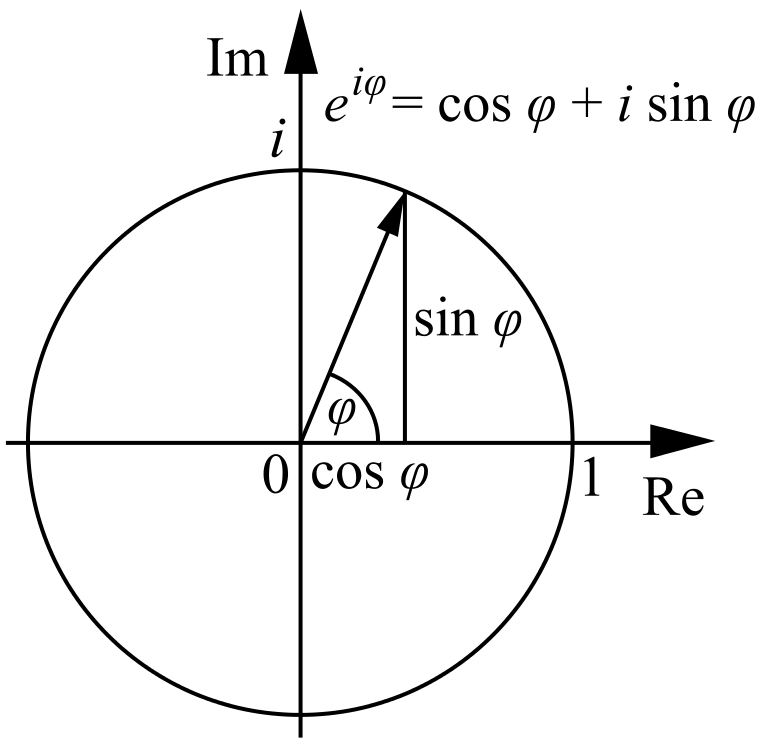
\includegraphics[width=0.5\textwidth]{euler.png}
\end{figure}
\end{frame}

\begin{frame}
\frametitle{Poles and zeros}
In general, the transfer function can be written as:
\begin{equation*}
H(s) = \frac{N(s)}{D(s)}.
\end{equation*}
\pause
The poles of $H(s)$ are zeros of $D(s)$, ie $\{s\ :\ D(s) = 0\}$.\\
\begin{itemize}
\item $|H(s)|=\infty$ if $s$ is a pole.
\end{itemize}
\ \newline
\pause
The zeros of $H(s)$ are zeros of $N(s)$, ie $\{s\ :\ N(s) = 0\}$. \\
\begin{itemize}
\item $H(s)=0$ if $s$ is a zero.
\end{itemize}
\pause
\ \newline
Poles and zeros may cancel, ie. if $D(s)=N(s)=0$ for some $s$.
\end{frame}

\begin{frame}
\frametitle{Steady-state response}
The output of a linear time-invariant system yields consists of:
\begin{itemize}
\item a steady-state output $y_{ss}(t)$, which similar periodicity to $u(t)$ \\
$\rightarrow$ $y_{ss}$ comprises the same frequencies as $u(t)$ \\
\item a transient output $y_{tr}(t)$ \\
$\rightarrow$ if the system is stable, then $\lim_{t\rightarrow\infty} y_{tr}(t) = 0$  \\
$\rightarrow$ $y_{tr}(t)$ depends on the initial state $\mathbf{x}_0(t)$ of the system
\end{itemize}
\pause
\ \newline
If we apply an input $u(t) = cos(\alpha t + \theta)$, then:
\begin{equation*}
y_{ss}(t) = |H(j\alpha)|cos(\alpha t + \theta + \angle H(j\alpha))
\end{equation*}
\pause
The steady-state output $y_{ss}(t)$ of a linear time invariant system:
\begin{itemize}
\item consists of signals of same frequencies as the input signal $u(t)$
\item which may have been magnified and/or phase changed
\end{itemize}
\end{frame}

\subsection{Impulse response and time constant}

\begin{frame}
\frametitle{Impulse response}
The impulse response $h(t)$ of input $i$ to output $j$ is the output $y_j(t)$ of a system when an impulse $\delta(t)$ is applied at input $u_i(t)$.\\
\ \newline
\pause
The impulse response is the inverse Laplace transform of the transfer function $h(t) = \mathcal{L}^{-1}\{H(s)\}$.\\ 
\ \newline
\pause
For stable continuous time systems the impulse response always converges to $0$:
\begin{equation*}
\lim_{t\rightarrow\infty} h(t) = 0, \text{ because } \mathbf{D}=0 \text{ and }\lim_{t\rightarrow\infty} \mathbf{x}(t) = 0.
\end{equation*}
\pause
The speed of convergence depends on the position of the poles.
\end{frame}

\begin{frame}
\frametitle{Time constant}
The transfer function of first order systems can be written as:
\begin{equation*}
H(s) = \frac{K}{\tau s + 1}\quad \leftrightarrow \quad h(t) = \frac{K}{\tau} e^{-t/\tau},
\end{equation*}
where $\tau$ is called the system's \textbf{time constant}.\\
\ \newline
\pause
The time constant summarizes the speed of a system's dynamics:
\begin{itemize}
\item after $\tau$ seconds, the impulse response reaches $h(0)/e$.
\item after $\tau$ seconds, the step response has reached $1-e^{-1}\approx63\%$ of its regime value.
\end{itemize}
\end{frame}

\begin{frame}
\frametitle{Impulse response $H(s)=5/(5s+1) \leftrightarrow h(t)=exp(-t/5)$}
\begin{figure}
\centering
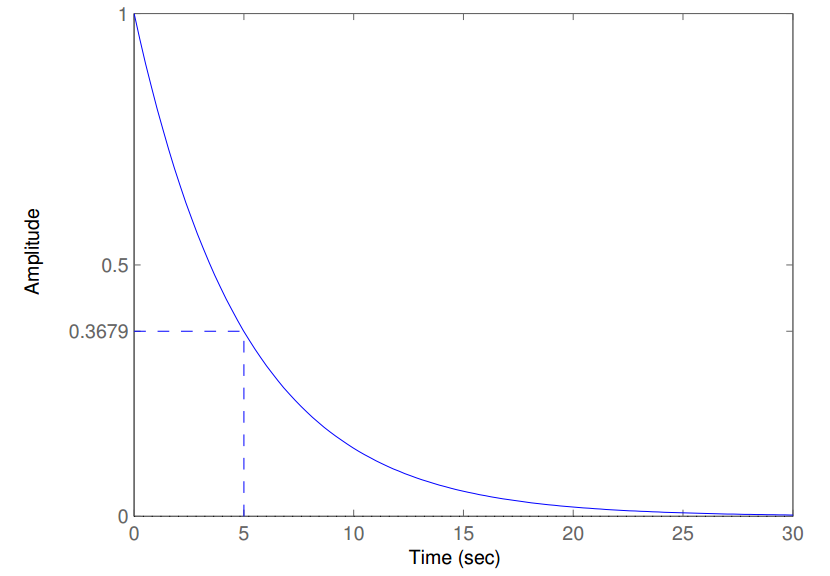
\includegraphics[width=0.8\textwidth]{time-constant-impulse.png}
\end{figure}
\end{frame}

\begin{frame}
\frametitle{Step response $H(s)=5/(5s+1) \leftrightarrow h(t)=exp(-t/5)$}
\begin{figure}
\centering
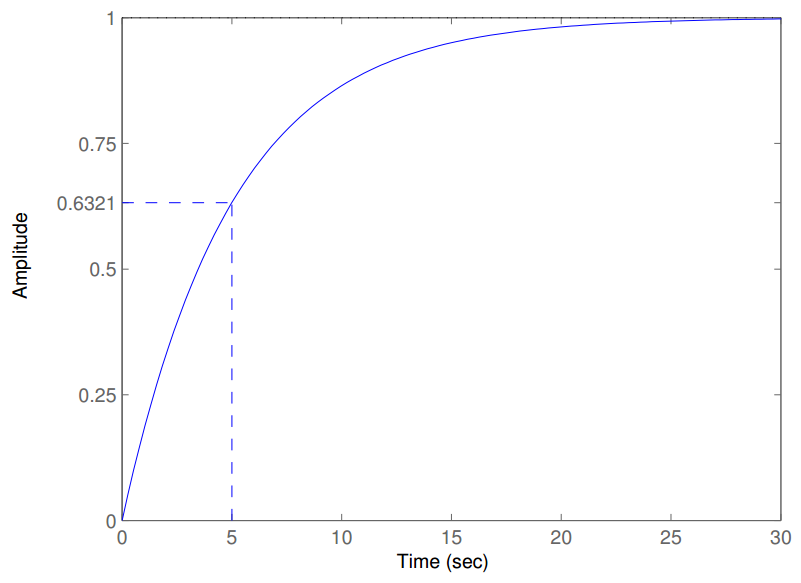
\includegraphics[width=0.8\textwidth]{time-constant-step.png}
\end{figure}
\end{frame}

\subsection{Relationship between state space and transfer functions}

\begin{frame}
\frametitle{From state-space to transfer functions}
We start from the linear state-space representation:
\begin{align*}
&\text{time domain}\hfill &\text{Laplace domain} \\
&\left\{ \begin{matrix}
\dot{\mathbf{x}}(t) = \mathbf{A} \mathbf{x}(t) + \mathbf{B} \mathbf{u}(t) \\
\mathbf{y}(t) = \mathbf{C} \mathbf{x}(t) + \mathbf{D} \mathbf{u}(t)
\end{matrix} \right. \quad\leftrightarrow\quad
&\left\{ \begin{matrix}
s \mathbf{X}(s) = \mathbf{A} \mathbf{X}(s) + \mathbf{B} \mathbf{U}(s) \\
\mathbf{Y}(s) = \mathbf{C} \mathbf{X}(s) + \mathbf{D} \mathbf{U}(s)
\end{matrix} \right.
\end{align*}
\pause
A transfer function $\mathbf{H}(s) = \frac{\mathbf{Y}(s)}{\mathbf{U}(s)}$ relates an input and an output in the Laplace-domain $\rightarrow$ to obtain it, we must eliminate $\mathbf{X}(s)$.
\pause
\begin{align*}
(s\mathbf{I}-\mathbf{A}) \mathbf{X}(s) &= \mathbf{B} \mathbf{U}(s) \\
\mathbf{X}(s) &= (s\mathbf{I}-\mathbf{A})^{-1} \mathbf{B} \mathbf{U}(s) \\
\Rightarrow \mathbf{Y}(s) &= \mathbf{C} (s\mathbf{I}-\mathbf{A})^{-1} \mathbf{B} \mathbf{U}(s) + \mathbf{D} \mathbf{U}(s) \\
\Rightarrow \hfill {\color{blue}\mathbf{H}(s)} &= {\color{blue}\mathbf{C} (s\mathbf{I}-\mathbf{A})^{-1} \mathbf{B} + \mathbf{D}}
\end{align*}
\end{frame}

\begin{frame}
\frametitle{Relationship between poles and eigenvalues of $\mathbf{A}$ 1/2}
Poles are zeros of the denominator of $\mathbf{H}(s)$, e.g. those values of $s$ for which $\mathbf{H}(s)$ is singular.\\ \pause
\ \newline
The relationship between state-space representation (matrices $\mathbf{A}$, $\mathbf{B}$, $\mathbf{C}$ and $\mathbf{D}$) and transfer functions is given by
\begin{equation*}
\mathbf{H}(s) = \mathbf{C} (s\mathbf{I}-\mathbf{A})^{-1} \mathbf{B} + \mathbf{D}
\end{equation*}
\pause
$H(s)$ cannot be computed when $(s\mathbf{I}-\mathbf{A})^{-1}$ does not exist, ie.
\begin{align*}
\det(s\mathbf{I}-\mathbf{A}) = 0
\end{align*}
\pause
The determinant is zero if $s$ is an eigenvalue of $\mathbf{A}$.\\ \pause
$\rightarrow$ {\color{blue}all poles of $\mathbf{H}(s)$ are eigenvalues of $\mathbf{A}$}
\end{frame}

\begin{frame}
\frametitle{Relationship between poles and eigenvalues of $\mathbf{A}$ 2/2}
Transfer functions only capture what is relevant to describe an input-output relationship, but not all states necessarily contribute.\pause\\
$\rightarrow$ \emph{unobservable} modes of $\mathbf{A}$ are not poles in $\mathbf{H}(s)$. \\
\pause
\ \newline
Consider the following SISO system with 2 states:
\begin{align*}
\begin{bmatrix} sX_1(s) \\ sX_2(s) \end{bmatrix} &= \begin{bmatrix} \alpha & 0 \\ 0.2 & 1 \end{bmatrix} \begin{bmatrix} X_1(s) \\ X_2(s) \end{bmatrix} + \begin{bmatrix} \beta \\ 2 \end{bmatrix} U(s) \\
Y(s) &= \begin{bmatrix} 1 & 0 \end{bmatrix} \begin{bmatrix} X_1(s) \\ X_2(s) \end{bmatrix}
\end{align*}
\pause
The transfer function $H(s) = \frac{\beta}{s-\alpha}$ has only one pole ($s_1 = \alpha$). \\
$\rightarrow$ {\color{blue}not all eigenvalues of $\mathbf{A}$ are poles in transfer functions $\mathbf{H}(s)$.}
\end{frame}

\end{document}
